\chapter{Парсинг реальных CAPTCHA для создания датасета}

Большинство предобученных моделей компьютерного зрения, таких как YOLOv8, обучены на датасете COCO~\cite{COCO}, содержащем изображения высокого качества с чёткими контурами и однозначной аннотацией объектов. Однако CAPTCHA с изображениями имеют принципиально иные характеристики: они могут включать в себя размытие, наложенные артефакты, искажения, шумы, повторяющиеся элементы и искусственно пониженное разрешение. Всё это снижает эффективность использования стандартных датасетов и моделей, не адаптированных под такие условия.

Для обеспечения высокой точности в задаче автоматического решения CAPTCHA необходимо подготовить собственный набор данных, приближённый к реальным условиям использования. Наиболее эффективным методом является автоматизированный парсинг изображений CAPTCHA, представленных на веб-сайтах, использующих визуальные CAPTCHA-решения, такие как Google reCAPTCHA v2.

\section{Преимущества парсинга реальных CAPTCHA}

Использование реальных CAPTCHA, собранных в автоматическом режиме, имеет ряд преимуществ по сравнению с синтетической генерацией данных:

\begin{enumerate}
    \item изображения содержат разнообразные сцены, освещение, углы обзора и уровни шума, что положительно влияет на способность модели к обобщению;
    \item присутствует большое количество уникальных объектов на фоне, в том числе в частично перекрытых и смазанных вариантах;
    \item отсутствует необходимость в ручной генерации изображений и создании дополнительных искажений для повышения реалистичности;
    \item возможно извлекать текстовые инструкции к CAPTCHA, что позволяет соотносить каждое изображение с требуемым классом.
\end{enumerate}

\section{Автоматизация сбора данных}

Для парсинга CAPTCHA был реализован автоматизированный сценарий взаимодействия с браузером с использованием библиотеки Selenium~\cite{Selenium}. Данный подход позволяет воспроизвести действия пользователя при работе с CAPTCHA, обходя при этом ручной ввод. Для обеспечения стабильной работы и масштабируемости процесса применялась браузерная автоматизация через WebDriver (в частности, ChromeDriver).

Функциональность парсера включает следующие ключевые этапы:

\begin{enumerate}
    \item поиск iframe-элемента, содержащего чекбокс <<Я не робот>>, и эмуляция клика по нему для инициирования визуальной CAPTCHA;
    \item ожидание загрузки CAPTCHA и извлечение изображения с заданием (включая его URL или пиксельный снимок);
    \item извлечение информации о структуре сетки (количество строк и столбцов), на которую разбито изображение CAPTCHA;
    \item получение текста задания, содержащего имя объекта (например, <<выберите все изображения с мотоциклами>>), для последующего использования в аннотации данных.
\end{enumerate}

Типичная CAPTCHA представляет собой изображение, разделённое на сетку из 3×3 или 4×4 ячеек, каждая из которых может содержать фрагмент сцены. При этом пользователю предлагается выбрать ячейки, в которых присутствует объект заданного класса. Процесс парсинга может быть представлена блок-схемой на рис.~\ref{fig:captcha-flow}.

\begin{figure}[H]
    \centering
    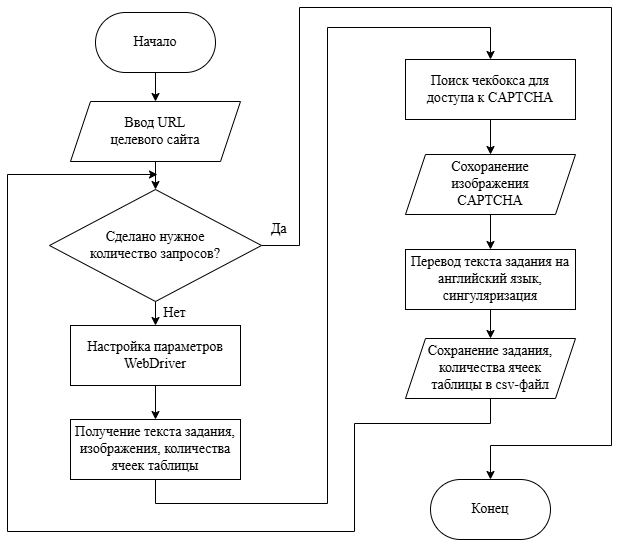
\includegraphics[width=0.65\textwidth]{imgs/image_captcha_flow.png}
    \caption{Блок-схема процесса парсинга CAPTCHA.}
    \label{fig:captcha-flow}
\end{figure}
\vspace{-0.5cm}

Полученные изображения и метаданные (включая текст задания и параметры сетки) используются для формирования обучающего датасета, пригодного для дообучения модели YOLOv8 в задачах классификации и сегментации объектов.
